% Created 2022-06-30 Thu 15:36
% Intended LaTeX compiler: pdflatex
\documentclass[11pt]{article}
\usepackage[utf8]{inputenc}
\usepackage[T1]{fontenc}
\usepackage{graphicx}
\usepackage{longtable}
\usepackage{wrapfig}
\usepackage{rotating}
\usepackage[normalem]{ulem}
\usepackage{amsmath}
\usepackage{amssymb}
\usepackage{capt-of}
\usepackage{hyperref}
\author{Mihir, Noah, Alfred}
\date{\today}
\title{Kontinuierliche Wahrscheinlichkeitsräume}
\hypersetup{
 pdfauthor={Mihir, Noah, Alfred},
 pdftitle={Kontinuierliche Wahrscheinlichkeitsräume},
 pdfkeywords={},
 pdfsubject={},
 pdfcreator={Emacs 28.1 (Org mode 9.6)}, 
 pdflang={English}}
\begin{document}

\maketitle
\tableofcontents


\section{Kontinuierliche Zufallsvariablen}
\label{sec:org8b7e25c}
\subsection{Definition 79}
\label{sec:org43482c7}
Eine kontinuierliche oder auch stetige Zufallsvariable \(X\) und ihr zugrunde liegender kontinuierlicher (reeller) Wahrscheinlichkeitsraum sind definiert durch eine integrierbare Dichte(-funktion) \\
\(f_X : \mathbb{R} \rightarrow \mathbb{R}^+_0\) mit der Eigenschaft \\
\(\sum_{-\infty}^{+\infty} f_X(x) dx = 1\) \\
\subsubsection{Verteilungsfunktion:}
\label{sec:orge7a7a35}
\(F_X(x) := Pr[X \leq x] = Pr[\{t \in R | t \leq x\}] = \int^x_{-\infty} f_X(t) dt\).
\subsection{Kolmogorov-Axiome und \(\sigma\)-Algebren}
\label{sec:org64e2f3d}
\subsubsection{\(\sigma\)-Algebren}
\label{sec:orge4bd135}
\begin{enumerate}
\item Definition 82
\label{sec:org34f858d}
Sei \(\Omega\) eine Menge. Eine Menge \(A \subseteq P(\Omega)\) heißt \(\sigma\)-Algebra über \(\Omega\), wenn folgende Eigenschaften erfüllt sind:
\begin{itemize}
\item (E1) \(\Omega \in A\).
\item (E2) Wenn \(A \in A\), dann folgt \(\bar{A} \in A\).
\item (E3) Für \(n \in \mathbb{N}\) sei \(A_n \in A\). Dann gilt auch \(\bigcup_{n=1}^\infty A_n \in A\)
\end{itemize}
\end{enumerate}
\subsubsection{1.3.2 Kolmogorov-Axiome}
\label{sec:orgcb9bb52}
Sei \(\Omega\) eine beliebige Menge und A eine \(\sigma\)-Algebra über \(\Omega\). Eine Abbildung \\
\(Pr[.] : A \rightarrow [0, 1]\) \\
heißt Wahrscheinlichkeitsmaß auf A, wenn sie folgende Eigenschaften besitzt:
\begin{itemize}
\item (W1) \(Pr[\Omega] = 1\)
\item (W2) A1, A2, . . . seien paarweise disjunkte Ereignisse. Dann gilt
\(Pr[\bigcup_{i=1}^\infty A_i] = \sum_{i=1}^\infty Pr[A_i]\)
\end{itemize}

\subsubsection{Lemma 84}
\label{sec:org2f7c2e8}
Sei \((\Omega, A, Pr)\) ein Wahrscheinlichkeitsraum. Für Ereignisse \(A, B, A_1, A_2,...,A_n\) gilt
\begin{itemize}
\item \(Pr[\emptyset] = 0, Pr[\Omega] = 1\)
\item \(0 \leq Pr[A] \leq 1\)
\item \(Pr[\bar{A}] = 1 − Pr[A]\)
\item Wenn \(A \subseteq B\), so folgt \(Pr[A] \leq Pr[B]\).
\item Bei paarweisen disjunkten Ereignissen A,B gilt \(Pr[A \cup B] = Pr[A] + Pr[B]\)
\end{itemize}

\subsection{Rechnen mit Kontinuierlichen Zufallsvariablen}
\label{sec:org347a828}
\subsubsection{1.4.1 Funktionen kontinuierlicher Zufallsvariablen}
\label{sec:org3d1b3c4}
Sei \(Y := g(X)\) mit einer Funktion \(g : R \rightarrow R\). \\
Die Verteilung von \(Y\) erhalten wir durch \\
\(F_Y(y) = Pr[Y \leq y] = Pr[g(X) \leq y] = \int_C f_X(t) dt\) \\
Hierbei bezeichnet \(C := {t \in R | g(t) \leq y}\)
\subsubsection{Kontinuierliche Zufallsvariablen als Grenzwerte diskreter Zufallsvariablen}
\label{sec:orgd79ab91}
Wir können aus einer kontinuierlichen Zufallsvariable \(X\) leicht eine diskrete Zufallsvariable konstruieren, indem wir für ein festes \(\delta > 0\) definieren \\
\(X_\delta = n\delta \iff X \in [n\delta, (n + 1)\delta[\) für \(n \in \mathbb{Z}\). \\
Für X\textsubscript{\(\delta\)} gilt \\
\(Pr[X_\delta = n_\delta] = F_X((n + 1)\delta) − F_X(n\delta)\) \\
\begin{center}
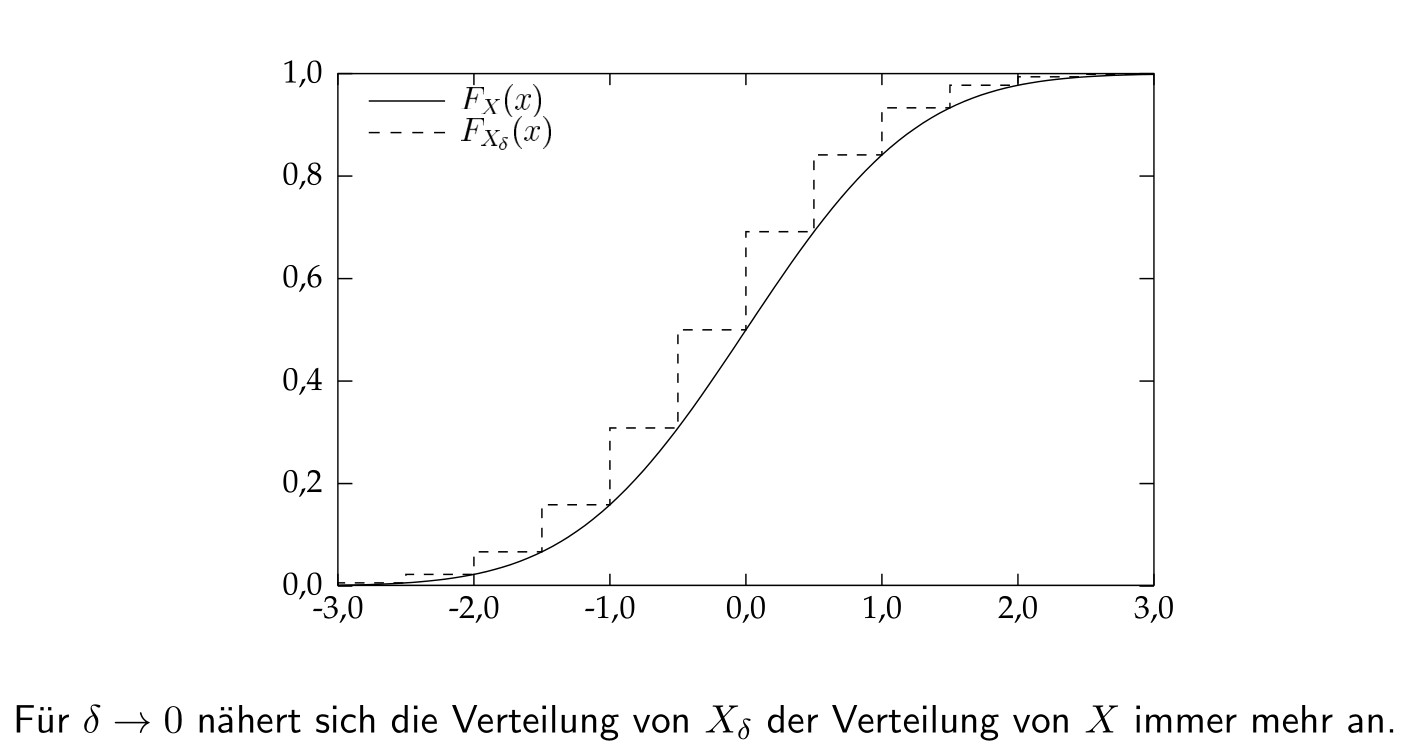
\includegraphics[width=.9\linewidth]{./img/Kontinuierliche_Wahrscheinlichkeitsräume/kontinuierliche_vs_diskrete_variablen.png}
\end{center}
\subsubsection{Erwartungswert und Varianz:}
\label{sec:orgecab294}
\begin{itemize}
\item \(E[X] = \int_{-\infty}^\infty t * f_X(t) dt\) sofern \(\int_{-\infty}^\infty |t| * f_X(t) dt\) endlich ist
\item \(Var[X] = E[(X - E[X])^2] = \int_{-\infty}^\infty (t - E[X])^2 * f_X(t) dt\) sofern \(E[(X - E[X])^2]\) existiert
\end{itemize}
Für \(Y = g(X)\) gilt: \\
\(E[Y] = \int_{-\infty}^\infty g(t) * f_X(t) dt\)

\section{Wichtige Stetige Verteilungen}
\label{sec:org2e59e22}
\subsection{Gleichverteilung}
\label{sec:orge86781e}
\(f_X(x) = \left\{ \begin{array}{ll} \frac{1}{b-a} & x \in [a,b] \\ 0 & sonst \\ \end{array} \right\) \\
\(F(x) = \int_{-\infty}^x f(t)dt = \left\{ \begin{array}{ll} 0 & x < a \\ \frac{x-a}{b-a} & a \leq x \leq b \\ 1 & x > b \\ \end{array} \right\) \\
\(E[X] = \frac{a+b}{2}\) \\
\(Var[X] = \frac{(a-b)^2}{12}\)
\subsection{Normalverteilung}
\label{sec:org51e25eb}
Eine Zufallsvariable X mit Wertebereich \(W_X = R\) heißt normalverteilt mit den Parametern \(\mu \in \mathbb{R}\) und \(\sigma \in \mathbb{R}^+\), wenn sie die Dichte \\
\(f(x) = \frac{1}{\sqrt{2\pi}\sigma} * exp(-\frac{(x - \mu)^2}{2\sigma^2}) =: \varphi(x;\mu,\sigma)\) \\
In Zeichen schreiben wir \(X \sim N(\mu, \sigma^2)\). \\
\(N(0, 1)\) heißt Standardnormalverteilung. Die zugehörige Dichte \(\varphi(x; 0, 1)\) kürzen wir \(\varphi(x)\) ab
\subsubsection{Verteilungsfunktion:}
\label{sec:orgc3b6df1}
\(F(x) = \frac{1}{\sqrt{2\pi}\sigma} * \int_{-\infty}^{x} exp(-\frac{(t - \mu)^2}{2\sigma^2}) dt =: \Phi(x;\mu,\sigma)\) \\
\subsubsection{Satz 93 (Lineare Transformation der Normalverteilung)}
\label{sec:orgbef842d}
Sei \(X\) eine normalverteilte Zufallsvariable mit \(X \sim N(\mu, \sigma^2)\). Dann gilt für beliebiges \\
\(a \in \mathbb{R} \backslash {0}\) und \(b \in \mathbb{R}\), dass \(Y = aX + b\) normalverteilt ist mit \(Y \sim N(a\mu + b, a^2\sigma^2)\) .
\subsubsection{Satz 94}
\label{sec:org632f590}
\(X\) sei \(N(0, 1)\) -verteilt. Dann gilt
\(E[X] = 0\) und
\(Var[X] = 1\).
\subsubsection{Satz 95}
\label{sec:org4fdc159}
\(X\) sei \(N(\mu, \sigma^2)\) -verteilt. Dann gilt
\(E[X] = \mu\) und \(Var[X] = \sigma^2\) .
\subsection{2.3 Exponentialverteilung}
\label{sec:org5e658d8}
\(f(x) = \left\{ \begin{array}{ll} \lambda * e^{-\lambda x} & x \geq 0 \\ 0 & sonst \\ \end{array} \right\) \\
\(F(x) = 1 - e^{-\lambda x}\) für \(x \geq 0\) \\
\(E[X] = \frac{1}{\lambda}\) \\
\(Var[X] = \frac{1}{\lambda^2}\) \\
\subsubsection{Satz 97 (Skalierung exponentialverteilter Variablen)}
\label{sec:orgf08ced8}
Wenn \(X\) exponentialvertielt ist mit \(\lambda\), so ist auch \(Y = aX\) mit \(a>0\) exponentialvertielt mit Parameter \(\lambda/a\)
\subsection{Satz 98 (Gedächtnislosigkeit)}
\label{sec:orgc725514}
Eine (positive) kontinuierliche Zufallsvariable \(X\) mit Wertebereich \(\mathbb{R}^+\) ist genau dann exponentialverteilt, wenn für alle \(x, y > 0\) gilt, dass \\
\(Pr[X > x + y | X > y] = Pr[X > x]\)

\section{Mehrere kontinuierliche Zufallsvariablen}
\label{sec:org3b62f20}
\subsection{Mehrdimensionale Dichten}
\label{sec:org2e94c00}
\(\int_{-\infty}^{\infty} \int_{-\infty}^{\infty} f_{X,Y}(x,y) dx \ dy= 1\)
\subsubsection{Randverteilung}
\label{sec:orge35593b}
\(F_X(x) = Pr[X \leq x] =\int_{-\infty}^x [\int_{-\infty}^\infty f_{X,Y} (u, v) dv]du\) \\
analog \\
\(f_X(x) = \int_{-\infty}^{\infty} f_{X,Y} (x, v) dv\)
\subsubsection{Unabhängigkeit}
\label{sec:org44fd8b1}
\(Pr[X \leq x, Y \leq y] = Pr[X \leq x] * Pr[Y \leq y]\) \\
gleichbedeutend \\
\(F_{X,Y} (x, y) = F_X(x) * F_Y(y)\) \\
Differentiation ergibt \\
\(f_{X,Y} (x, y) = f_X(x) * f_Y (y)\)
\subsection{3.3 Warteprobleme mit der Exponentialverteilung}
\label{sec:orgd61f778}
Die Zufallsvariablen \(X_1,... , X_n\) seien unabhängig und exponentialverteilt mit den Parametern \(\lambda_1, ... , \lambda_n\). Dann ist auch \(X := min\{X_1, . . . , X_n\}\) exponentialverteilt mit dem Parameter \(\lambda_1 + ... + \lambda_n\).

\subsection{Poisson-Prozess}
\label{sec:orgf6ad4de}
\begin{itemize}
\item Wenn der zeitliche Abstand der Treffer geometrisch verteilt ist, so ist ihre Anzahl in einer festen Zeitspanne binomialverteilt.
\item Wenn man Ereignisse zählt, deren zeitlicher Abstand exponentialverteilt ist, so ist die Anzahl dieser Ereignisse in einer festen Zeitspanne Poisson-verteilt.
\end{itemize}

\subsection{Summen von Zufallsvariablen}
\label{sec:orga150ab5}
Seien \(X\) und \(Y\) unabhängige kontinuierliche Zufallsvariablen. Für die Dichte von \(Z := X + Y\) gilt \\
\(f_Z(z) =\int_{-\infty}^\infty f_X(x) * f_Y (z − x) dx\)
\subsubsection{Satz 106 (Additivit¨at der Normalverteilung)}
\label{sec:orgf930621}
Die Zufallsvariablen \(X_1,..., X_n\) seien unabhängig und normalverteilt mit den Parametern \(\mu_i, \sigma_i (1 \leq i \leq n)\) \\
Es gilt: Die Zufallsvariable \\
\(Z := a_1X_1 + ... + a_nX_n\) \\
ist normalverteilt mit Erwartungswert \(\mu = a_1\mu_1 + ... + a_n\mu_n\) und Varianz \(\sigma^2 = a^2_1\sigma^2_1+ ... + a^2_n\sigma^2_n\)
\subsection{3.5 Momenterzeugende Funktionen für kontinuierliche Zufallsvariablen}
\label{sec:orgff26a97}
Für diskrete Zufallsvariablen \(X\) haben wir die momenterzeugende Funktion \\
\(M_X(s) = E[e^{Xs}]\)
eingeführt. Diese Definition kann man unmittelbar auf kontinuierliche Zufallsvariablen übertragen. Die für \(M_X(s)\) gezeigten Eigenschaften bleiben dabei erhalten. \\
\(M^{(k)}_X(0) = E[X^k]\)

\section{Zentraler Grenzwertsatz}
\label{sec:orgce0736b}
Die Zufallsvariablen \(X_1, ... , X_n\) besitzen jeweils dieselbe Verteilung und seien unabhängig. Erwartungswert und Varianz von \(X_i\) existieren für \(i = 1, ... , n\) und seien mit \(\mu\) bzw. \(\sigma^2\) bezeichnet (\(\sigma^2 > 0\)).
Die Zufallsvariablen \(Y_n\) seien definiert durch \(Yn := X_1 + . . . + X_n\) für \(n \geq 1\). Dann folgt, dass die Zufallsvariablen \\
\(Z_n := \frac{Y_n - n\mu}{\sigma \sqrt{n}}\) \\
asymptotisch standardnormalverteilt sind, also \(Z_n \sim N(0, 1)\) für \(n \rightarrow \infty\)

\subsubsection{Intuitive Konsequenz:}
\label{sec:org48c7490}
Wenn eine Zufallsgröße durch lineare Kombination vieler unabhängiger, identisch verteilter Zufallsgrößen entsteht, so erhält man näherungsweise eine Normalverteilung

\subsection{Korollar 109 (Grenzwertsatz von de Moivre)}
\label{sec:org2a18370}
\(X_1, ... , X_n\) seien unabhängige Bernoulli-verteilte Zufallsvariablen mit gleicher Erfolgswahrscheinlichkeit \(p\). Dann gilt für die Zufallsvariable \(H_n\) mit \\
\(H_n := X1_ + ... + X_n\)
für \(n \geq 1\), dass die Verteilung der Zufallsvariablen \\
\(H^∗_n := \frac{H_n - np}{\sqrt{np(1 - p)}}\) \\
für \(n \rightarrow \infty\) gegen die Standardnormalverteilung konvergiert.

\section{Normalverteilung als Grenzwert der Binomialverteilung}
\label{sec:org38040c3}
\subsubsection{Korollar 110}
\label{sec:orgc120d3a}
Sei \(H_n \sim Bin(n, p)\) eine binomialverteilte Zufallsvariable. Die Verteilung von \(H_n/n\) konvergiert gegen \(N(p, p(1 − p)/n)\) für \(n \rightarrow \infty\)
\subsection{Verschiedene Approximationen der Binomialverteilung}
\label{sec:org3c9a5ff}
Sei \(H_n \sim Bin(n, p)\) eine binomialverteilte Zufallsvariable mit der Verteilungsfunktion \(F_n\) . Für \(n \rightarrow \infty\) gilt \\
\(F_n(t) = Pr[H_n/n \leq t/n]\)
\(\rightarow \Phi (\frac {t/n - p}{\sqrt{p(1 - p)/n}}) = \Phi (\frac {t - np}{\sqrt{p(1 - p)n}})\)

Wir können \(F_n\) somit für große \(n\) durch \(\Phi\) approximieren. Diese Approximation ist in der Praxis deshalb von Bedeutung, da die Auswertung der Verteilungsfunktion der Binomialverteilung für große \(n\) sehr aufwändig ist, während für die Berechnung der Normalverteilung effiziente numerische Methoden vorliegen.

\section{Approximationen für die Binomialverteilung}
\label{sec:org2b79605}
\begin{itemize}
\item Approximation durch die Poisson-Verteilung: \(Bin(n, p)\) wird approximiert durch \(Po(np)\). Diese Approximation funktioniert sehr gut für seltene Ereignisse, d. h. wenn \(np\) sehr klein gegenüber \(n\) ist. Als Faustregel fordert man \(n \geq 30\) und \(p \leq 0,05\).
\item Approximation durch die Chernoff-Schranken: Bei der Berechnung der tails der Binomialverteilung liefern diese Ungleichungen meist sehr gute Ergebnisse. Ihre Stärke liegt darin, dass es sich bei den Schranken nicht um Approximationen, sondern um echte Abschätzungen handelt. Dies ist vor allem dann wichtig, wenn man nicht nur numerische Näherungen erhalten möchte, sondern allgemeine Aussagen über die Wahrscheinlichkeit von Ereignissen beweisen möchte.
\item Approximation durch die Normalverteilung: Als Faustregel sagt man, dass die Verteilungsfunktion \(F_n(t)\) von \(Bin(n, p)\) durch \\
\(F_n(t) \approx \Phi((t - np)/ \sqrt{p(1 - p)n})\) \\
approximiert werden kann, wenn \(np \geq 5\) und \(n(1 - p) \geq 5\) gilt.
\end{itemize}
\end{document}
